\chapter{Conclusions}
\label{Chapter6}
\lhead{Chapter 6. \emph{Conclusions}}

\begin{figure}[H]
  \centering
  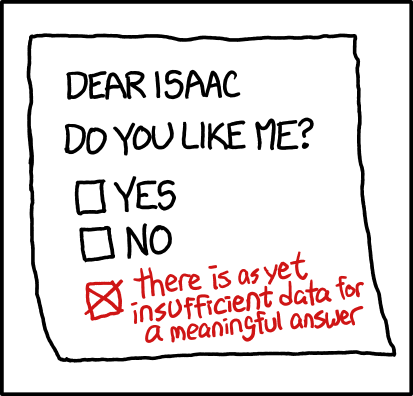
\includegraphics{Figures/xkcd/chapter6.png}
  \caption*{xkcd.com/1448}
\end{figure}

In this thesis, I aimed to demonstrate the ability to photometrically classify SLSNe amongst large samples of transients detected by modern, wide-field astronomical surveys. In order to achieve this, I combined our understanding of this class of objects with state-of-the-art Machine Learning and light curve modelling techniques to both define and predict their behaviour in a number of surveys. All this was performed with the aim of broadening our understanding of SLSNe as a population. The main results are summarised below.

\section{Modelling SN light curves}
In \cref{Chapter3}, I described the methods for modelling of CCSN and SLSN. I discussed the analytical models as well as the tools built to implement them. I have learned a number of lessons regarding the problems with modelling of both classes, as outlined in this chapter. I also describe the Bayesian approach to the problem of model optimisation and introduces Gaussian Process Regression as a tool for non-parametric, probabilistic light curve interpolation.

\subsection{Modelling SLSNe}
The simulations of SLSNe at any chosen redshift or bandpass were essential for this thesis. In \sref{sec:SLAP}, I demonstrated an approach to producing a high-quality SLSN SED model based on the black-body approximation of its continuum, combined with a spectral absorption template. The templates, focusing on the UV regions of the SED, significantly increased the redshift range at which it is possible to confidently model these objects. I combined this with the evolution of the bolometric luminosity of SLSNe based on the birth and spin-down of a magnetar model, modified to include a variable opacity term. I showed that this treatment of SLSNe correctly accounts for their light curve morphology including the late time evolution which is difficult to capture using other models.

\subsection{Modelling CCSN}
While CCSN are a better-understood class of transients than SLSNe, their simulation tools are still underdeveloped, especially when compared to those used for the modelling of SN\,Ia. Here, I developed a set of tool for simulating CCSNe, including both their hydrogen-poor and rich subclasses. I provide a self-contained solution, starting with the archival photometric and spectroscopic data for a number of nearby objects of these classes. After a number of models are trialled, I use an approach similar to \citet{Bazin2009} in order to provide an interpolation model used to flux calibrate the observed spectra in the process referred to as mangling. Based on this approach, I built \textsc{CoCo}, a tool for generating spectral templates and simulations of CCSNe.

The approach used in this thesis works on the principle of placing a spectral template at any required redshift, then passing it through a bandpass filter to measure the synthetic flux at the phases of the spectra before fitting a light curve model to them to obtain flux at any arbitrary point. Due to the wavelength limitations of ground-based spectroscopy, the SED had to be extended in both IR and UV regimes. I used a combination of auxiliary \textit{Swift}-UVOT data and the modelling of their continuum as dust extinct black-bodies to achieve a wavelength coverage reaching as low as $\sim1500\AA$, sufficient to obtain the flux of a CCSN in the DES \textit{g}-band at their detection limit of z$\sim$0.7.

\subsection{Light Curve interpolation using Gaussian Processes}
Throughout this thesis, I used GPR as a method for light curve interpolation. Upon comparing a number of popular covariance functions, I determined that the Mate\'rn 3/2 kernel best suits the light curve data familiar to this work. I found it to be the best overall match to all classes of SN detected by DES and a good fit to highly variable objects such as AGNs, that form a large fraction of the transients observed by DES. This approach has been shown to successfully fit all transients in the artificial and well as DES transients samples, demonstrating its robustness.

\section{Rates of SLSN}
\cref{Chapter4} of this thesis focused on measuring the rate of SLSNe at the intermediate redshift of z$\sim$1. This was motivated by the low numbers of similar measurements, despite being a crucial piece of the puzzle of the origin on SLSNe. In this work, I provide one of the most accurate measurements of the rate, allowing us for the first time, to probe its evolution with redshift as well as the connection to other rare classes of transients.

\subsection{Defining SLSNe}
Starting from the SLSN model, based on the spin-down of a magnetar, I postulated a definition the SLSNe. After fitting the literature sample of these objects with the model, I found all SLSNe to concentrate in a small region of the P$_{ms}$-B$_{14}$-$\mathrm{\tau}_M$ parameter space, clearly separated from a majority of transients detected my SNLS. I parametrised this region using an ellipsoid that tightly encapsulates the entire training sample, giving a definition of SLSNe in terms of the parameter space of the magnetar model.

\subsection{Search for SLSN in SNLS}
I used this proposed definition of SLSNe to search for the presence of new, previously unclassified objects in the SNLS. Upon fitting the entire archival sample of transients, taking either their precise spectroscopic redshift (where available) or a range of host galaxy photometric redshift estimates, I find that only two new objects fall within my definition. While one of them shows clear signs of multiseason variability, the second object, SNLS07D3bs, was found to be a strong SLSN candidate. My modelling suggested a good match to the class at 0.6$<$z$<1$. Using a low Sn\/N, archival spectrum of the object we were unable to confirm the classification, however, we used narrow line features to determine the true redshift of the object as z=0.74, confirming that the object is consistent with the luminosity of a SLSN.

\subsection{Rate of SLSNe at z$\sim$1}
With three SLSN candidates found in the SNLS, I performed a Monte Carlo simulation of the survey, replicating its transient detection behaviour. This reversed the common approach of calculating the rate of SNe by weighing each object by its detection efficiency and observed volume. Instead, I simulated SLSNe before applying the survey noise and measuring each objects detectability in the survey. In the simulations, I iterated over a range of rate values, measuring the resulting number of SLSN detections. I then transpose these results to give me the probability of detecting 3 objects as a function of the input value. I found the rate of SLSNe, at z$\sim$1, to be $91^{+76}_{-36}$\,SNe\,Yr$^{-1}$\,Gpc$^{-3}$ or 2.2$^{+1.8}_{-0.9}\times10^{-4}$ of the CCSN rate. This is consistent with similar publications and tentatively demonstrates that the rate of SLSNe follows that of the cosmic star formation rate.

\subsection{Connection between SLSNe and ULGRBs}
An interesting question probed in \citet{Prajs2016} is the connection between the classes of SLSNe and ULGRBs. LGRB are known to be connected to ordinary, stripped-envelope SNe which, under certain circumstances, result in the formation of a collapsar, or a jet forming young black hole powered by the infalling ejecta. Thanks to the advances in GRB observation provided by the \textit{Swift} satellite, we now know that some LGRB are observed to emit $\gamma$-radiation bursts lasting up to 10,000s \citep{Levan2013a}. A correction has been recently drawn between this class of ULGRBs and SLSNe, thanks to the discovery of GRB\,111209A. Observed simultaneously as SN2011kl, a SN with a luminosity, light curve morphology and spectroscopic characteristics similar to other lower luminosity SLSNe \citep{Greiner2015}.

ULGRB are known to be rarer than ordinary LGRBs with their exact rate difficult to estimate due to the \textit{Swift} observations and GRB triggering mechanism being optimised to detect short transients, likely leading to a loss of many potential candidates. In \citet{Prajs2016}, we have approximated the rate of ULGRBs based on the estimates of the key components of the measurement. Taking 10 years of \textit{Swift} observations, detecting ULGRBs up to z$\sim1.3$ with a 17\% sky coverage an approximate detection and classification efficiency of 30\% we find the rate of ULGRBs to be $\rho_{\mathrm{ULGRB}} \sim 30~\mathrm{Gpc}^{-1} \mathrm{yr}^{-1}$. In contrast to SLSNe, this measurement depends on the beam angle of the $\gamma$-emission as GRBs do not radiate isotropically. We used an opening angle of $\theta=12^\circ$ which can be seen as a conservative estimate, in line with the other values used here, resulting in this estimate to be seen as a lower limit on the true rate. Regardless, it is of particular interest that the value estimated for both SLSNe and ULGRBs appear very close, perhaps giving more evidence to their intrinsic connection and a shared physical origin.

\section{Photometic classification of SN}
Photometric classification of SNe forms the centre piece of this thesis. Performed using a number of methods, I demonstrate that the ML approach is the most powerful and successful, albeit, not the most straightforward to implement solution. While it required the construction of a large, artificial training sample, the results obtained using this method have largely exceeded the capabilities of other tools publically available to date.

\subsection{Training sample}
Using the combination of readily available models for SN\,Ia and AGNs as well as custom build models of SLSNe and CCSN, I have built a large training sample of transient light curves. I applied survey noise and cadence to match its properties with the real DES transient sample. The final sample consisted of $\sim$300,000 objects, therefore being the largest to date light curve collection used for a photometric classification study and represents objects from low redshift, local objects to those that lay at the edge of DES detectability.

\subsection{Machine Learning Model}
I developed a two-stage approach to the problem of classifying DES transients in order to reduce the number of free parameter in the model. In the first step, I separate SNe (regardless of their class) from other contaminants in the sample, including AGNs and spurious noise detections. This focuses on long-term variability of the object rather than their detailed evolution, used in the next stage to subdivide the SN sample
into their respective classes. This approach produces an excellent classification rate, correctly identifying 99.81\% SNe in the training sample. This was verified using a ground-truth sample where all spectroscopically confirmed transients (SNe and AGN) were correctly identified in this work.

Similarly to the SN identification pipeline, the SN classification algorithm exceeded our accuracy expectations. Compared to other similar projects, I did not use the spectroscopic redshift as a classification prior but, with a 97.85\% classification rate, I achieved a higher precision than reported by the current state-of-the-art solution \citep{Lochner2016}. Upon identifying the sample of DES SNe, consisting of 5273 objects, I tested the model against a ground-truth sample of spectroscopically confirmed SN\,Ia, correctly identifying 243 out of 250 objects. It is even more encouraging to mention that the misclassified objects formed extreme season edge cases where no data was observed near the maximum light for these objects.

Applying this technique to the full sample of DES transients, I identified 3120 potential SN\,Ia as well as 509 SLSN candidates. The later number vastly exceeded our expectations based on the rate of SLSNe measured in \cref{Chapter4}. The visual inspection of the data showed that the sample is heavily contaminated by SN\,IIP, with characteristic long, red and plateauing light curves. We can attribute this to the lack of similar objects in the training sample as no objects of this class have passed the quality cuts required to generate a \textsc{CoCo} template

\subsection{Selecting SLSN}
Starting with a sample of 509 potential SLSN candidates, I used the auxiliary information on the objects including their host galaxies spectroscopic and photometric redshift measurements to analyse the sample, producing a pure sample of viable SLSN candidates. I used the redshifts measured by the AAT instrument to select 26 objects with an absolute luminosity, in its brightest photometric band, greater than M$_{mathrm{max}}~<~$-19.5.

Amongst this sample, I discovered 10 SLSN candidates in the first season of DES where only one candidate has previously been known, solving one of the big mysteries of the DES sample of SLSNe. However, no objects have been identified at redshift comparable or exceeding that of DES16C2nm demonstrating the need for a deeper analysis of the objects selected here and a development of more robust models of SN\,IIP that could be used to inform the ML classification tools.

\section{Future Work}
Having developed a successful approach for the photometric classification of SLSNe in large astronomical surveys, there are a number of avenues that I would like to pursue in the future. This includes the improvement and application of the method to in other surveys as well as using the archival data to solve some of the yet to be explained mysteries of SLSNe.

\subsection{Expanding the Training Sample}
One of the biggest issues identified in the process of photometrically classifying SLSNe was the incompleteness of the SN sample used in the training of the ML algorithm. The lack of examples of SN\,IIP had the greatest effect as it introduces a large number of impurity in the sample of SLSNe. However, the lack of other classes including rapidly evolving SNe and Tidal Disruption events also means that we cannot treat the samples of photometrically identified SN\,Ia and CCSNe as a pure sample.

In this thesis, the training sample was based on the spectroscopic templates for each class generated from the archival data for some of their most well-observed examples. While the techniques have generally varied in details, they all required spectroscopic data to an extent. However, for a number of classes or rare and fast transients, spectroscopy is very scarce while their photometries remain relatively abundant. A new approach, not requiring such extensive commitment from the data, is needed to extend the training samples. A possible solution, requiring a large commitment of resources, would be to use physically motivated simulations to produce a sample of objects and test their similarity to the available photometric samples. This approach is likely the most viable for the problem of modelling SN\,IIP where we could base the modelling on the existing simulations \citep{Dessart2013,Dessart2016}.

\subsection{Rates of SLSNe from DES}
A natural extension of the work undergone in \cref{Chapter4} is to use the sample of SLSNe found in \cref{Chapter5} to compute their rate. The increase from 3 to 43 objects, compared to SNLS, would result in a vastly decreased uncertainties in the overall measurement. More importantly, it will be the first-ever measurement allowing for a separation of the rate into separate redshift bins using a single, homogeneous sample. With a tenfold increase in the observing area of the survey, the computational resources required to calculate the rate using the approach used in SNLS would likely be prohibitive. However, as part of the process of building the artificial sample of SLSNe, I simulated a large number of the randomly generated object throughout DES. While the main objective of this was to generate a sample of detectable SLSNe, the detection efficiency for each artificial SN is a by-product of this process. This gives us the tools necessary to calculate the detection efficiency of DES SLSNe by comparing their magnetar model fits those of the artificial sample.

\subsection{Selecting SLSN in LSST}
In the upcoming decade, LSST will dominate the landscape of optical astronomy and change the way that astronomers approach data reduction and selection of candidates for further follow-up. It is predicted that $\sim$10,000 SLSNe will be detected by the survey every year in the shallow fields as the longer cadence and all-sky coverage are ideal for the detection of these slowly evolving SNe. However, with such high number of objects and the millions of possible contaminants, the traditional non-ML methods of photometric classification would be too computationally prohibitive, as well as likely not effective.

The method proposed in \cref{Chapter5} is a promising approach to the problems faced by LSST, however, a pure CNN approach can only be directly used with relatively long light curves making it impossible to target these objects for spectroscopic follow-up during their early rise-time phases. One possible extension that may be introduced to the current method is the use of the intermediate layers of the CNN as a way of identifying the light curve features which are most indicative of SLSNe. While this is not as powerful as a full CNN treatment, it would largely decrease the number of potential candidates and along with other auxiliary information, including the host galaxy properties and redshift.

\subsection{Redshift estimation for photometric SN\,Ia in DES}
Perhaps one of the most interesting results in this thesis, not directly related to the main subject of SLSNe, is the accuracy of the photometric classification of SN\,Ia. This is likely a reflection on the maturity of the model used to build the training sample of this class as well as our understanding of its parameter spaces. The lack of use of a redshift prior in the ML classification was motivated by the majority of objects in the real DES transient sample not being associated with an accurate redshift measurement. However, this information is present for each artificially generated light curve and could be used to estimate the redshift of the real DES SN\,Ia. This proposed new method would not require its estimation from model fitting but could be learned directly from the data given a sufficiently large data set.

\section{Final remarks}
The field of SLSNe research is still in its early stages. With the upcoming era of LSST, the numbers of SN detections are going to change the way we approach their properties, shifting fully from the study of individual objects to their statistical properties as a whole. We do not, however, have to wait until the LSST first light to begin this work. In this thesis, I demonstrated that the number of SLSNe detected by DES, each containing a high quality light curves and a wealth of supplementary data, by the nature of the survey, likely exceeds the total number of SLSNe discovered prior to DES. There are still a number of hidden secrets in the data, including many SLSN at z $\sim$ 2 waiting to be discovered by the next generations of ML algorithms.
